\documentclass[12pt,titlepage,final]{article}
\usepackage{graphicx}
\usepackage{mathtools}
\begin{document}
\graphicspath{{./images/}}
\title{\textsc{Modern Interferometry Lab}}
\author{Anthony Ford, Alex Garcia, Rossina Miller}
\date{November 30, 2011}
\maketitle

\begin{abstract}
The objective of this experiment was to assemble a Michelson Interferometer,
experiment with different ways of viewing the interference patterns, and explore
methods of measuring the alignment and achieving optimum alignment. We were able
to properly construct and align our Michelson Interferometer, achieving a
visibility close to 1.
\end{abstract}

\section{Theory}

The purpose of this experiment is to see how an interferometer works. The
Michelson interferometer is the design that will be used for the experiment. A
Michelson interferometer is a simple interferometer that is used to make very
small and precise measurements, in fact the Michelson interferometer is the
layout used in LIGO\@. A Michelson interferometer works by having a laser shoot
down a path into a beam splitter that splits the laser beam into two seperate
paths. At the end of each path there is a mirror that will reflect the laser
back toward the beam splitter which then combines the two beams. After the
recombination the lasers will be either in or out of phase, due to the
superposition principle. The superposition principle basically says that when
two waves pass through the same point in space their amplitudes will combine;
this causes the net amplitude to add or subtract, known as constructive and
destructive interference respectively. Constructive interference happens if the
waves are in phase while destructive interference happens when the waves are out
of phase.

\begin{figure}[ht!]
\centering
%Caption: Two waves in phase and the next is two waves 180 degress out of phase
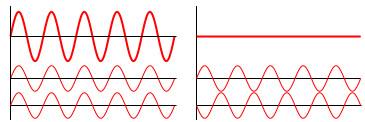
\includegraphics[width=4 in]{Interference_of_two_waves}
\caption{Two waves in phase and the next is two waves 180 degrees out of phase}
\end{figure}

In this experiment the only way that the phase will change will be due to the distance between the mirrors and the beam splitter. The phase difference,$\Delta \phi$, is calculated by 
	\begin{align}
		\nonumber \Delta \phi &=\frac{2\pi}{\lambda} \Delta p
	\end{align}
with $\Delta p$ being the difference in the paths and $\lambda$ being the wavelength of the laser being used. From there we can then say that 
	\begin{align}
		\nonumber \Delta p &=\sum(n_2 d_2)-\sum(n_1 d_1) \\
		\nonumber		&=n_2 d_2 - n_1 d_1
	\end{align} 
where $d$ is the distance from the beam splitter to the cube and $n$ is index of refraction of the medium the beam is traveling through. For this experiment the medium's are the same, they are both traveling through air, so then $n_1=n_2$ which results in
	\begin{align}
		\nonumber \Delta p &= n_2 d_2 - n_1 d_1 \\
		\nonumber 	&= n(d_2 - d_1) \\
		\nonumber \Delta \phi &=\frac{2\pi n}{\lambda} (d_2 - d_1)
	\end{align}

The change in phase will then affect the intensity of the beam, causing fringes to appear. These fringes will be red and black rings on a screen or piece of paper behind the lens. The black rings signify a destructive interference while the red rings are due to the constructive interference. 

Using a photodiode to get the fringes to appear on an oscilloscope it is then possible to get the voltage required to move from one fringe to another. Using this information with the properties of the piezo stack it is possible to get the wavelength of the laser. 




\section{Description}


We used various optics to build a Michelson Interferometer (a  complete list will be added at the end of this document.) We had to do several things during the process such as align the beam, mount some delicate optics, and test the end result. 

We mounted the He-Ne laser to the ULM-Tilt base and then placed it on one corner of the breadboard. This was done in such a way as to align the laser beam with the holes on the breadboard. We then had to assemble the silver mirrors onto their mounts. Using slips of paper to stabilize each mirror in its respective mount, we secured them in place. The mounts themselves were then attached to posts and placed in the following locations, shown in the diagram below.

\begin{figure}[ht]
\centering
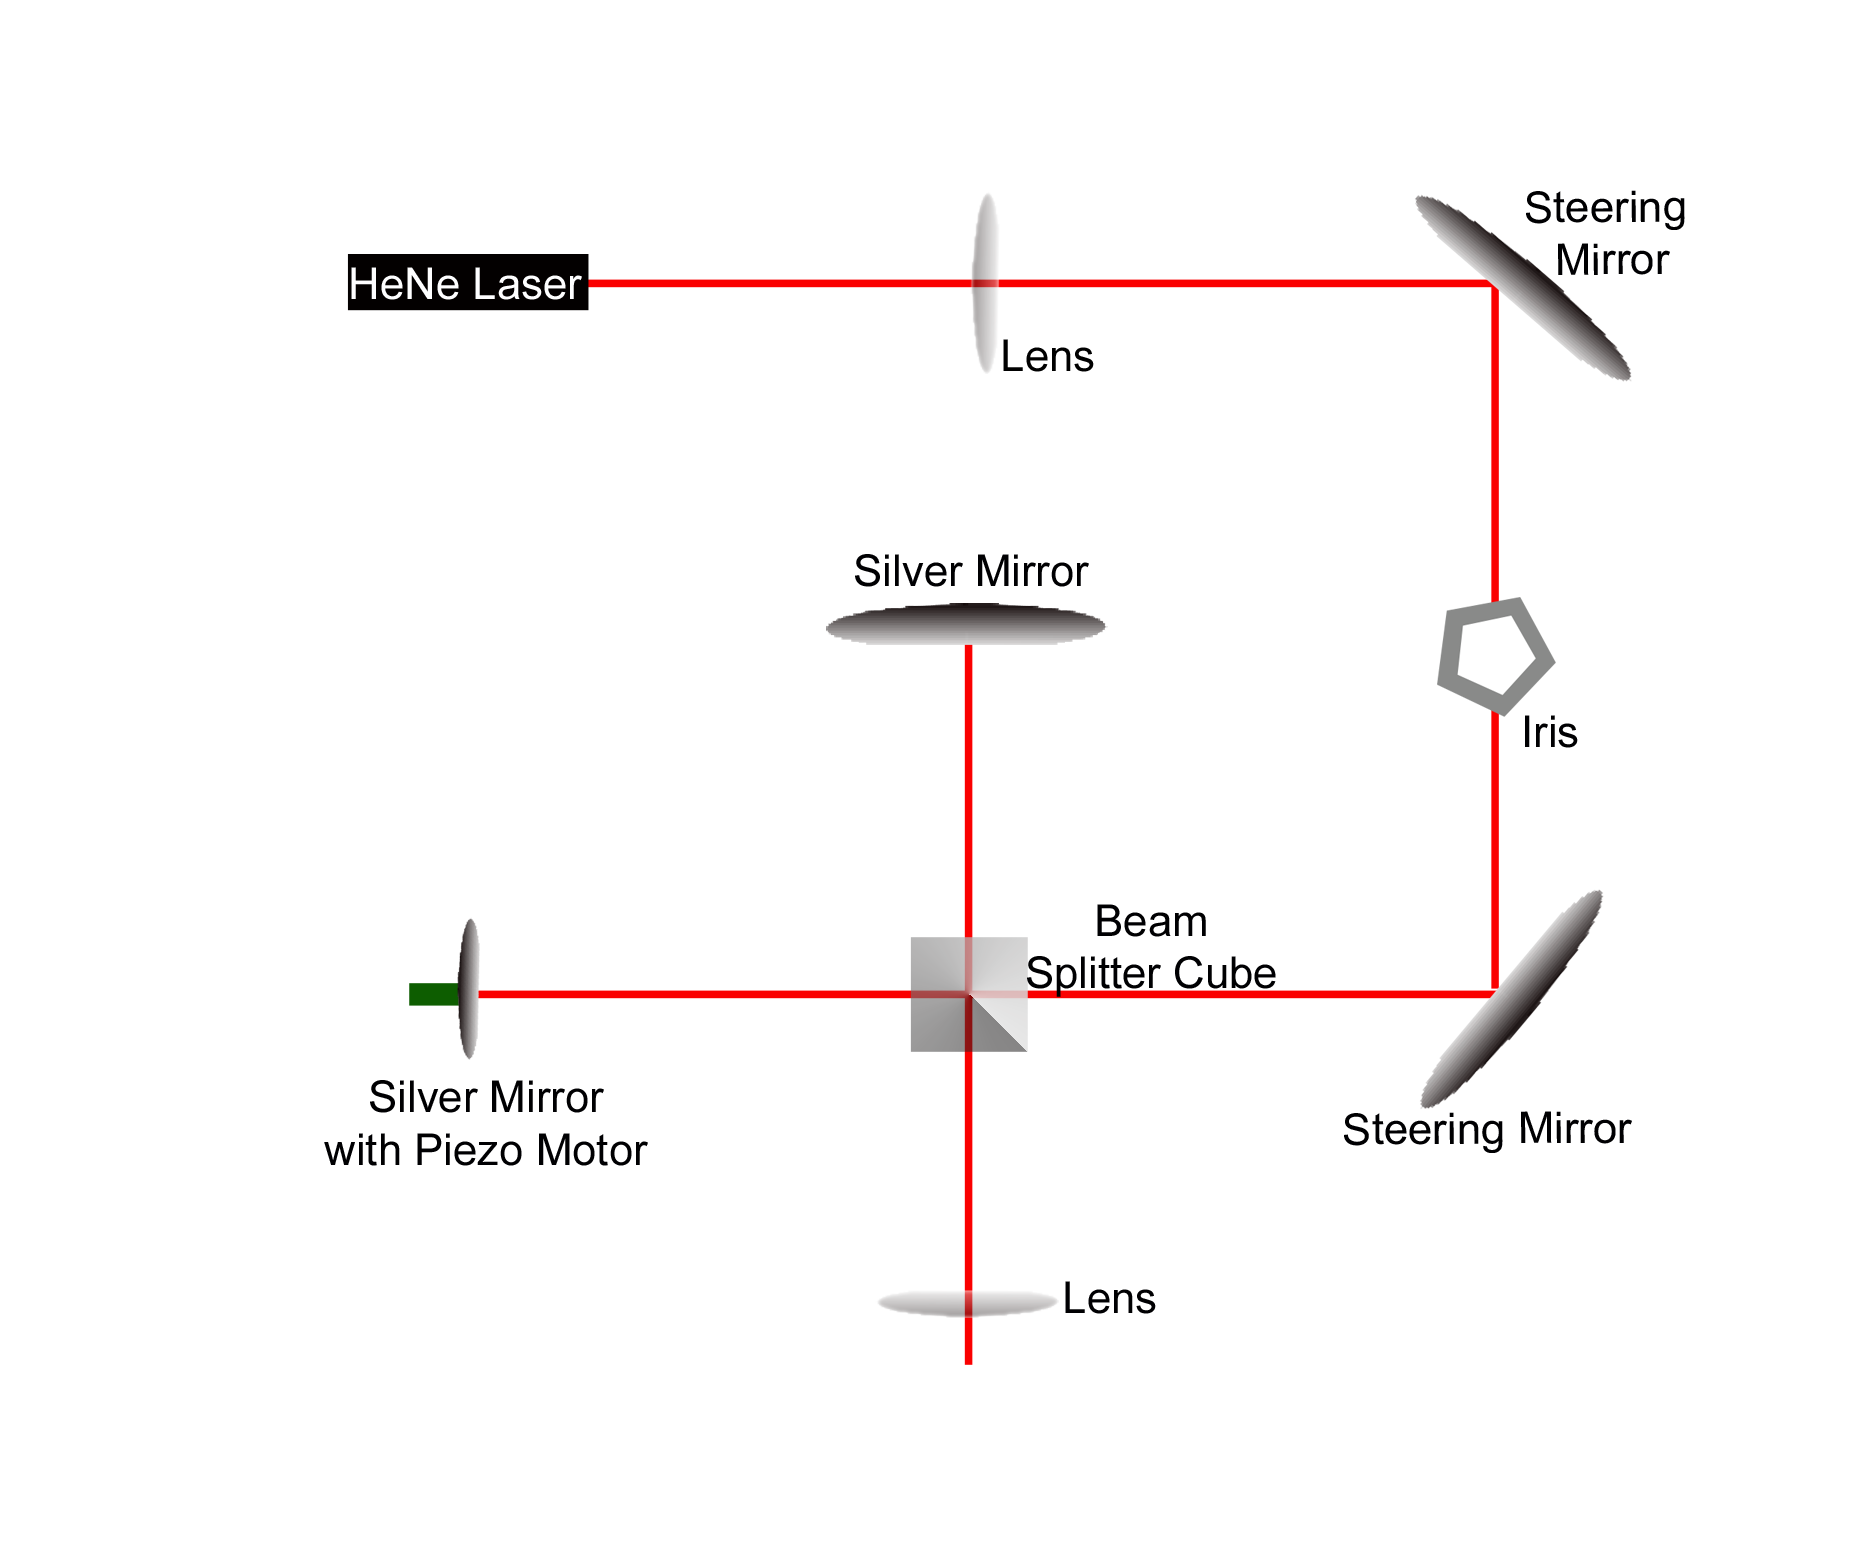
\includegraphics[width=5.5in]{interferometer}
\caption{Interferometer Diagram}
\label{fig:interferometer}
\end{figure}

The next major step we had to overcome was mounting the 0.5 in mirror on the piezo motor, but once in place we simply placed it on a post and set it aside.  Then we carefully mounted the beam splitter cube onto its mount with a small clamping arm. The mounted beam splitter was placed 4.5 inches away from Mirror 1 (the middle mirror in the diagram.) Using the same measurement we placed the Piezo Mirror to the left of the beam splitter.  After setting up this general layout, we turned on the laser to properly align it along the designated path.

The first step in aligning the beam, is to level it out. To do this we used an iris, set at height equal to the mirrors. We then placed the iris between the two steering mirrors to make sure the laser reflected back thru the iris opening. Minor adjustments of the mirrors were required to ensure this.  To obtain a level beam between the second steering mirror, the beam splitter and the piezo mirror the iris has to be moved along it path. First it is placed right in front of the steering mirror and then moved back to the beam splitter to see whether the beam is angled up or down. We once again made adjustments to the mirror until the beam was basically level. After this, the beam traveled from the steering mirror to thru the beam splitter to the Piezo Mirror and back without too much disparity. The beam splitter shoots off a secondary beam to Mirror 3, we just made minor adjustments to try and center this beam on the mirror. 

At this point we could see two splotches on the sheet of white paper that we placed after Lens 2. By making adjustments to Mirror 3, we were able place one splotch on top of the other and get an interference pattern. By looking at this interference pattern we were able to determine if we had correctly aligned the interferometer. An almost perfect or perfect alignment will yield a circular interference pattern, a black dot surrounded by rings or just rings. By pressing on the table (though had the instrument been less sensitive, by changing the arm lengths with a moving mount) we were able to push the interference pattern through several wavelengths at a time. In order to just move through one fringe set, we used the piezo mirror hooked up to a function generator and we replaced Lens 2 with a Photo Diode Detector which was hooked up to an oscilloscope.

Being careful not to send a square wave through the Piezo and keeping the frequencies below 100 Hz, we created a low frequency sinusoid on the function generator (Figure 2).

		\begin{figure}[ht!]
		\centering
		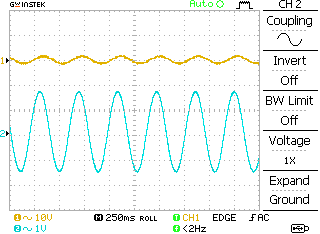
\includegraphics[width=4in]{DS0000}
		\caption{Low Frequency Sinusoid}
		\end{figure}

We then connected function generator's output to Channel 2 on the oscilloscope and to the Piezo via a T-connector. We then calculated the voltage difference that is required to move the Piezo Mirror through one fringe change or half a wavelength.

		\begin{figure}[ht!]
		\centering
		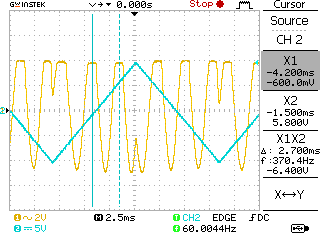
\includegraphics[width=4in]{DS0007}
		\caption{The yellow line represents the changes in the fringes as seen by the photo diode, and the blue line is the ramp function that is running to the Piezo.}
		\end{figure}

\section{Measurements}

\begin{tabular*}{1.16\textwidth}{| @{\hspace{.5cm}}r | @{\hspace{.5cm}}r | @{\hspace{.5cm}}r | @{\hspace{.5cm}}r 
				|@{\hspace{.5cm}}r  | @{\hspace{.5cm}}r | @{\hspace{.5cm}}r | @{\hspace{.5cm}}r || @{\hspace{.5cm}}r |}
	\hline
	$\Delta V_1$ & $\Delta V_2$ & $\Delta V_3$ & $\Delta V_4$ & $\Delta V_5$ & $\Delta V_6$ & 
	$\Delta V_7$ & $\Delta V_8$ & Avg $\Delta V$ \\
    \hline 
	6.0 V & 6.4 V & 5.4 V & 5.6 V & 6.6 V & 7.2 V & 3.6 V & 6.0 V &     5.85 V\\
    \hline
    6.2 V & 5.8 V & 6.4 V & 5.6 V & 7.2 V & 5.6 V & 7.0 V & 5.4 V &     6.15 V\\
	\hline

\end{tabular*}

\begin{tabular}{@{\extracolsep{\fill}}| c | c |}
	\hline
	$Y_1$ & $Y_2$ \\
	\hline
	4.40 & 4.15 \\
	\hline
\end{tabular} 

\section{Results/Analysis}
\begin{align*}
	\gamma &= \frac{I_{Max} - I_{Min}}{I_{Max} + I_{Min}} \\
	\gamma &= \frac{1 - -1}{1 + -1} \\
	\gamma &= 
\end{align*} 
The visibility from our interferometer was BLEH!! \\
The piezo moves 6.1 $\mu$m per 100 Volts so therefore it moves a total of 61 $\frac{\mu m}{V}$.
The value of $\Delta V_{averaged}$ comes from the average of the $\Delta V$.
\begin{align*}
	D &= \frac{\lambda}{2} \\
	D &= 61e^{-6} * \Delta V_{averaged} \\
	  &= 61e^{-6} * 6 \\
	D &= 366e^{-9} \\
	\lambda &= 2*D \\
	 &= 732e^{-9}	
\end{align*}
The wavelength of the laser comes out to be 739 $n$m. The actual value of the laser's wavelength is 632 $n$m, so our error was 
	\begin{align*}
		error &=\frac{\lambda_{real}-\lambda_{expected}}{\lambda_{real}} \\
			&= \frac{|632e^{-9}-732e^{-9}|}{632e^{-9}}	\\	
			&= 15.82
	\end{align*}


\section{Summary}
%Summarize, in a paragraph or two, what you conclude from the results of your
%experiment and whether they are what you expected them to be. Include brief
%answers to the specific questions asked in the lab instructions.

Throughout the course of this experiment, we discovered that interferometers are
more structurally simple than the thought, and much more sensitive than we had
anticipated.   


\subsection{Responses}
\begin{description}
    \item[Question 1] \hfill \\
        The visibility of this interferometer is 1.02, as calculated in
        Section~\ref{sec:results}.
    \item[Question 2] \hfill \\
        The experimental result shows that our laser has a wavelength of 732
        $nm$, a 15.82\% error when compared with the actual wavelength listed of
        632 $nm$.
    \item[Question 3] \hfill \\
        The action of striking or leaning on the table causes vibrations and
        deformations in the table's surface, changing the path length between
        each leg of the interferometer. This changes the phase difference
        between each leg, creating interference, and thus, fringes.
\end{description}


\section{Remarks}
%Please critique the experiment as presented in the lab manual. Could the lab be done in a better way? Do you have some other or original method for obtaining the same results? Your suggestions are encouraged and are used to improve the lab manual.

This lab definitely needs some improvement, should it be presented in this way again. With the addition of the lab manual building an interferometer will certainly be easier, however, having all the correct parts really is a must.  We had to borrow many pieces from the optics lab and even had to order some new parts. Time was a factor here, and had we more time we might have been able to create other experiments for students to test.  However all that being said, we were able to build an interferometer, align and measure changes in the interference pattern.

\end{document}
